% SETUP
\documentclass[11pt]{article}
\linespread{1.15}
\usepackage[english]{babel}
\usepackage[utf8]{inputenc}
\usepackage{graphicx, amsmath, array, graphics, amssymb, epsfig, psfrag, geometry, alltt, subfiles, blindtext, enumitem,float,pdfpages,multicol}
\usepackage[export]{adjustbox}
\usepackage{fancyhdr}
\usepackage{array}
\usepackage{hyperref}
%%%%%%%%%%%%%%  code listing
\usepackage{listings}
\usepackage{color} %red, green, blue, yellow, cyan, magenta, black, white
\definecolor{mygreen}{RGB}{2,94,33} % color values Red, Green, Blue
\definecolor{mylilas}{RGB}{170,55,241}
\usepackage{hyperref}
\hypersetup{
    colorlinks=true,
    linkcolor=black,
    filecolor=magenta,      
    urlcolor=blue,
}
\urlstyle{same}
%Includes "References" in the table of contents
\usepackage[nottoc]{tocbibind}

% MATLAB code insert
\lstset{language=Matlab,%
    %basicstyle=\color{red},
    breaklines=true,%
    morekeywords={matlab2tikz},
    keywordstyle=\color{blue},%
    morekeywords=[2]{1}, keywordstyle=[2]{\color{black}},
    identifierstyle=\color{black},%
    stringstyle=\color{mylilas},
    commentstyle=\color{mygreen},%
    showstringspaces=false,%without this there will be a symbol in the places where there is a space
    numbers=left,%
    numberstyle={\tiny \color{black}},% size of the numbers
    numbersep=9pt, % this defines how far the numbers are from the text
    emph=[1]{for,end,break},emphstyle=[1]\color{black}, %some words to emphasise
    %emph=[2]{word1,word2}, emphstyle=[2]{style},    
}
%%%%%%%%%%%%%%%%


\geometry{a4paper, top = 20mm, bottom = 20mm, left = 15mm, right = 15mm}

% Do we need a cover page?

% Headers
\pagestyle{fancy}
\fancyhf{}
\chead{ELEN90066 Embedded System Design - Final Report}
\cfoot{\thepage}

\begin{document}
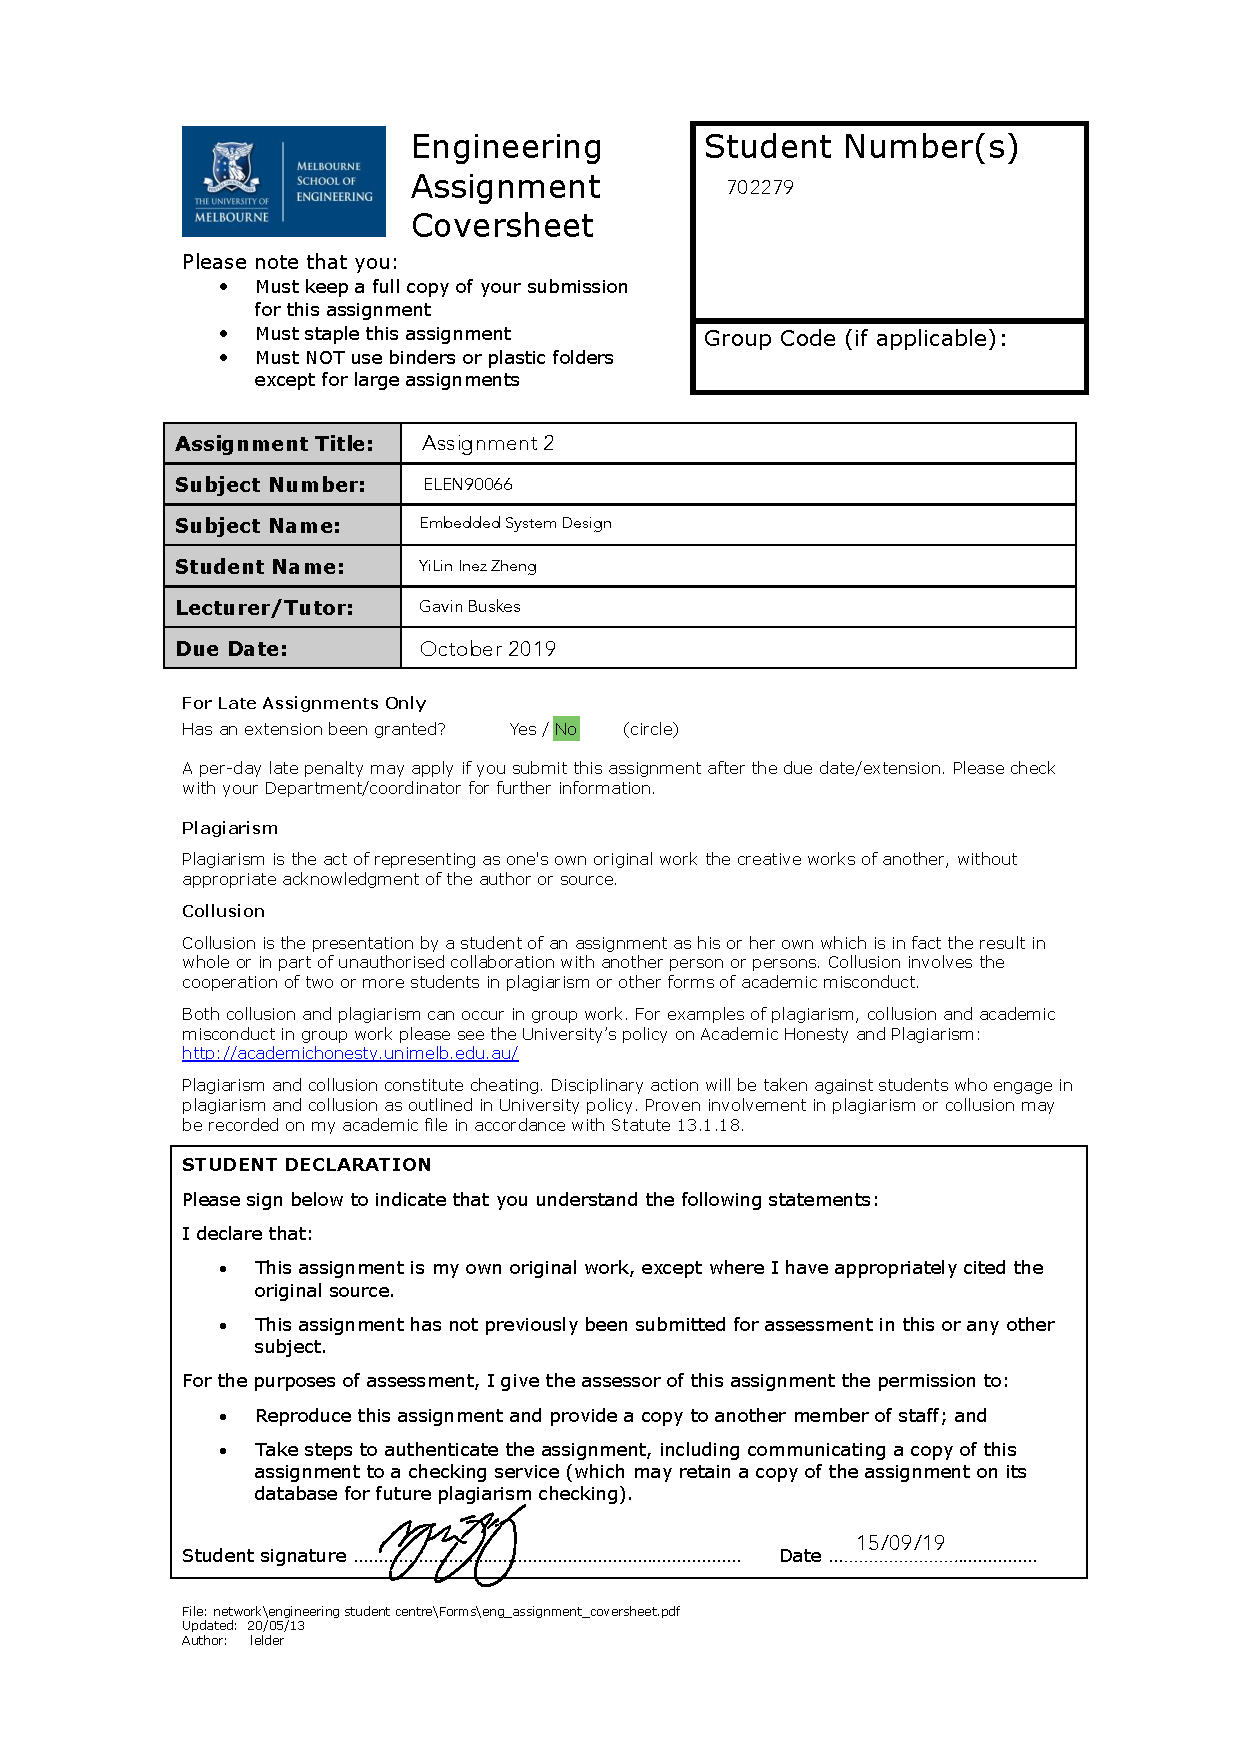
\includepdf{EngCSAss1.pdf}
\clearpage
\setcounter{page}{1}

% Title
\begin{center}
\textbf{\Large{Kobuki Obstacle Course Project - Final Report}}\\
Group 9: Craig Reid [756879], Xiuwen Peng [825801], YiLin Inez Zheng [702279], \\
Workshop: Monday 15:15pm - 18:15pm (Bigi), Due: 04/11/19  
\end{center}

%%% 20 page limit! %%%
\tableofcontents

\section*{Executive Summary}
%%% 150 words ish

\newpage
\section{Introduction}
The Kobuki is an educational "turtle-bot" designed with hardware robustness and long lasting battery life to supply power to external devices. This allows us to connect the Kobuki up to a \texttt{NI myRIO-1900} reconfigurable I/O device and use the FPGA for implementing designs of a finite state machine (FSM) that navigates the Kobui through a 3x5m obstacle course. The arrangement of the myRIO on the Kobuki is shown in the Figure \ref{fig:kobuki}. The legend to the bottom right corner of Figure \ref{fig:kobuki} shows the orientation of the accelerometer ADXL330 used in myRIO. The forward direction for the Kobuki is the positive $x$ axis. 
\begin{figure}[H]
    \centering
    \includegraphics[width=8cm]{Kobuki.png}
    \caption{30cm diameter Kobuki with connected myRIO in bird's eye view}
    \label{fig:kobuki}
\end{figure}

\subsection{Project Requirements}
To successfully complete the obstacle course, we must follow the following requirements and rules:
\begin{itemize}
    \item \textbf{Play/Pause}: 
    The Kobuki's action will be determined by it's 'B0' button. The robot shall only start when B0 is pressed. When pressed again all movement should be paused and the robot will resume upon another press of B0. The B0 button can also be referred to as the 'Play' button.
    \item \textbf{Driving}:
    The robot should stay level on the ground whilst moving at all times. The original positive $x$ axis position of the Kobuki at the start of the obstacle course determines the 'Ground Orientation', which the Kobuki should always follow. The ground orientation can only change after a power cycle, reprogram or restart of the robot or its embedded controller. There are also additional challenges to overcome whilst driving:
    \begin{itemize}
        \item \textbf{Obstacle Avoidance}:
        The Kobuki should always avoid obstacles in the form of cliffs, wheel hazards, and objects whilst driving even during simultaneous or shortly successive encounters. After encountering obstacles, the Kobuki must be able to reorient and resume driving in ground orientation. The Kobuki is allowed to touch objects as long as it changes course immediately to avoid the obstacle. 
        \item \textbf{Hill Climb}:
        The Kobuki must be able to climb up a hill, drive through the plateau and descend to a final stop on flat ground within 40cm of the bottom of the hill. The robot must be able to orient itself on the hill to execute an orthogonal climb or descent. At any time the robot must not go over the edge of the hill.
    \end{itemize}
    \item \textbf{Performance Specfications}
    \begin{itemize}
        \item \textbf{Rotation}: The Kobuki should not rotate more than 180 degrees.
        \item \textbf{Chattering}: Chattering and erratic movement should not be exhibited.
        \item \textbf{Abnormal Termination}: With the exception of power or mechanical failure, the robot should not stop at any time.
        \item \textbf{Obstacle Hugging}: The Kobuki is not allowed to repeated encounter the same obstacle for navigation.
        \item \textbf{Timeliness}: The obstacle course should be completed within 60 seconds.
    \end{itemize}
\end{itemize}

%%%% Design
\section{System Analysis and Design}\label{sec:system}
\vspace{-0.2cm} Exploring the complexity introduced by an unknown obstacle course led us to abstract key system features through variables and hence designing an Extended Finite State Machine (EFSM). Navigating the obstacle course using an EFSM allows flexibility in control and a level of autonomous decision making by the robot in response to sensor and actuator signals. To enable smarter controller design, whilst analysing the physical Kobuki, comparisons were also drawn with the available simulation environment, which is based on iRobot.

\subsection{Kobuki Sensors and Data}
%A basic description of the sensor data available to myRIO and how it was used in your algorithm
\vspace{-0.2cm} With a variety of sensors available on the Kobuki as shown in Figure \ref{fig:kobuki_sensors}, we chose to use applicable sensors for our obstacle navigation. Table \ref{table:kobuki_sensors} shows the sensors we used in our design and the obstacle course specifications that the sensors will help achieve. The wheel drop sensors and bumpers are both triggered as boolean outputs when the requirement of the wheel touching the ground or bumper uncollided is no longer true. The cliff sensor will avoid cliffs deeper than 5cm \cite{kobuki_datasheet}, the sensor range is 2 - 15cm \cite{kobukisensors}.
\begin{figure}[H]
    \centering
    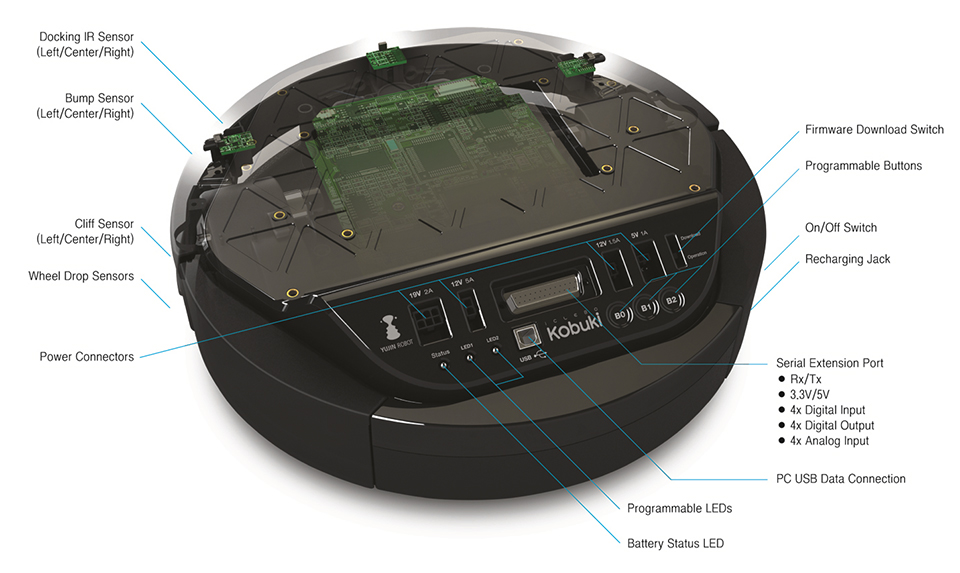
\includegraphics[width=12cm]{kobuki_spec.jpg}
    \caption{Angle view of Kobuki with sensors labelled \cite{kobuki_spec_pic}}
    \label{fig:kobuki_sensors}
\end{figure}
\begin{table}[H]
\begin{center}
\begin{tabular}{ |l|c|c|c| } 
    \hline
    \textbf{Sensor} & \textbf{Number} & \textbf{Target Specification} & \textbf{Output} \\ 
    \hline
    Wheel Drop Sensor & 2 (left, right) & Maintain ground contact & Boolean\\
    \hline
    Cliff Sensor & 3 (left, center, right) & Hill climb edge avoidance & Boolean and Raw\\
    \hline
    Bumper & 3 (left, center, right) & Object avoidance & Boolean\\
    \hline
\end{tabular}
\caption{Kobuki Sensors} \label{table:kobuki_sensors}
\end{center}
\end{table}
\vspace{-0.5cm}
The Kobuki polls the sensors at 50Hz and returns the above sensor data as default ``Basic Sensor Data" in the form of a hexadecimal bytestream \cite{kobukisensors}. These sensors were also available on the simulation environment iRobot though in different quantities. The iRobot has one extra wheel drop sensor due to the robot having an extra fourth wheel, one extra cliff sensor due to two front sensors (left, right), and one less centre bumper \cite{labguide}.\\

In addition to direct sensor data, the Kobuki also receives information on distance travelled (in mm) and angle rotated (in degrees) since origin. Compared to the simulation output, the real distance is signed and has angles unwrapped within $(-180^\circ, 180^\circ)$. The distance travelled is derived from the wheel movement so if the wheels were stuck but kept moving, the reported distance travelled will still increase. The simulation only records the actual distance moved by the robot in the sample environment \cite{labguide}. The maximum rotational velocity is $180^\circ$/s (anything above $110^\circ$ will see degraded gyro performance) and the maximum transitional velocity is 70cm/s \cite{kobuki_datasheet}. 

\subsection{Accelerometer ADXL330} \label{sec:acc}
\vspace{-0.2cm} In order to detect inclination and reorient the Kobuki on an incline, we used the accelerometer on the myRIO instead of the Kobuki gyroscope that is already used for determining rotation. The accelerometer offers a greater precision for readings in 3 axes ($x$, $y$, $z$) in comparison to the gyroscope's single axis reading. This will allow a greater sensitivity to the ground's incline environment. A\\

Using the accelerometer readings we calculate the pitch $(\theta)$ and yaw $(\psi)$ angles in radians with respect to the Kobuki axis orientation in Figure \ref{fig:kobuki} \cite{fisher_2011}. %Pitch is the same for both simulation and the Kobuki where from $+x$ towards $+z$ is increasing $\theta$ and from $+x$ towards $-z$ is decreasing $\theta$. Yaw is defined as increasing $\psi$ from $+x$ in the $-y$ direction and decreasing $\psi$ from $+x$ in the $+y$ direction. 
Figures X-X indicate the angles in context of the Kobuki and the resulting angle expressions in Eq.\ref{eq:accel_angles} are adapted from Fisher \cite{fisher_2011}. The yaw angle is calculated with a negative to allow efficient testing in simulation. The iRobot has the $\pm y$ directions swapped, where from $+x$ to $+y$ is increasing in $\psi$ and vice versa.
%% Insert drawings of angles!! 
\begin{align}\label{eq:accel_angles}
    \theta &= \arccos \biggr( \frac{z}{\sqrt{x^2 + y^2 + z^2}} \biggr)\\
    \psi &= \arctan(-\frac{y}{x})\\
\end{align}

\textcolor{blue}{TO DO:\\
- angle difference with simulation, smoother transition\\
- inclined compass reference\\
- thresholds\\
- sensitivty, ax + b equation thing}

\subsection{Design for Requirements}
%% methodology behind how we decided to tackle hill climb and obstacle avoidance
The two main design requirements of obstacle avoidance and hill climbing were designed separately to simplify the design process.  
\subsubsection{Obstacle Avoidance}
The obstacle avoidance algorithm was designed iteratively, each iteration addressed new use cases and problems from the previous iteration.
\begin{enumerate}
    \item The most basic design for obstacle avoidance is shown in Figure \#. When the Kobuki collided with an object it would simply reverse, rotate 90 degrees, travel parallel to the obstacle, rotate back and continue. This algorithm proved effective at travelling around obstacles, however would only rotate in one direction when avoiding. This resulted in the Kobuki rotating right even though it collided with an obstacle with the right bumper.
    \item The algorithm was improved by ensuring that the Kobuki rotated in the opposite direction to the obstacle. That is, if the right bumper was pressed then the Kobuki would avoid by rotating left. If the centre bumper was pressed, it simply rotated right. This algorithm proved to be much more effective at avoiding certain obstacles. However, there was still a risk of losing the initial heading. If the Kobuki hit an obstacle during the avoiding state it would simply reverse, rotate and avoid again. Clearly, this caused the initial orientation to be lost.
    \item The final iteration added the handling of meeting obstacles during the avoiding state. New states were added to ensure that the Kobuki would rotate back to the initial heading after reversing. Additionally, to avoid getting stuck in a corner a variable was added to change the direction that the Kobuki turned when the centre bumper was pressed.
\end{enumerate}

\subsubsection{Hill Climb}
The hill climbing algorithm also went through some iterations. The algorithms are based on the ability to detect an incline and then when on the incline, the ability to re-orient towards the top/bottom of hill. 
\begin{enumerate}
    \item The first hill climbing algorithm used the accelerometer data directly to detect a hill. An incline was detected when the $z$ accelerometer value decreased to below a certain threshold. Similarly, when on a hill, the Kobuki rotated until the $y$ accelerometer value decreased in magnitude below a certain threshold.
    \item Hill detection and hill orientation was greatly improved when the equations in Section \ref{sec:acc} were used. Additionally, to remove any bias in the accelerometer, when the Kobuki is first unpaused the sensor is effectively `zeroed'. This improved the reliability of detecting an incline. However, selecting a threshold for hill orientation that worked well without chattering was difficult.
    \item The final iteration radically changed the way the Kobuki reoriented on a hill. Instead of stopping and rotating until a threshold is met, a feedback loop was introduced. The relative speeds of each wheel were adjusted to be proportional to the difference between the current orientation and the desired orientation.
\end{enumerate}

\subsection{Final State Machine}
%A complete FSM diagram (including pause states) of the robot algorithm using the notation covered in the lectures. If you use an Extended state machine, or state refinements, you must show all states, variables and transitions.
There are 3 levels to the hierarchical extended state machine. The run/pause level, the obstacle avoidance level and the hill climbing level. When the system is in the run state, the system enters into the state refinement for obstacle avoidance. During the drive state of the obstacle avoidance refinement the system enters another state refinement to handle hill climbing. Note that the transitions to the states with refinements are history transitions - the refinements remember which state they are in rather than resetting. This is crucial for the pause behaviour and for tracking the hill states. This design neatly abstracts the different tasks that the Kobuki must perform. There is also the added benefit of being able to avoid obstacles while hill climbing - no additional states are required to avoid the cliffs. The state diagram is shown in Figure \ref{fig:FSM}. Trigger and action labels are used to simplify the diagram, see Tables \ref{tab:triggers} and \ref{tab:actions} for the label definitions. The output converter in Table \ref{tab:outputs} uses the variable \textit{DriveMode} to convert to the left and right wheel speeds on each update. The \textit{incline} and \textit{tiltAngle} variables are calculated on each update according to the pitch and yaw calculations of Section \ref{sec:acc}.\\ % did we want to label the tables too? to hyperreference?

\begin{figure}[p]
    \centering
    \begin{tabular}{ll}
      \textbf{inputs:}   & \textit{B0} : pure\\
                         & \textit{cliffLeft, cliffCentre, cliffRight} : pure \\
                         & \textit{bumpLeft, bumpCenter, bumpRight} : pure \\
                         & \textit{wheelDropLeft, wheelDropRight} : pure\\
                         & acc : $\mathbb{R}^3$\\
                         & \textit{netAngle, netDistance} : $\mathbb{R}$\\
      \textbf{variables:}& \textit{driveMode} : \{FORWARD, BACKWARD, ROTATE\_LEFT, ROTATE\_RIGHT, ARC, STOP\}\\
                         & \textit{incline, tiltAngle} : $\mathbb{R}$\\
                         & \textit{turnPct} : $\mathbb{R}$\\
                         & \textit{distance, angle} : $\mathbb{R}$\\
                         & \textit{obstacleLoc} : \{LEFT, CENTRE, RIGHT\}\\
                         & \textit{offsets} : $\mathbb{R}^3$\\
                         & \textit{centreTurn} : \{\textit{true, false}\}\\
     \textbf{outputs:}   & \textit{leftWheelSpeed}, \textit{rightWheelSpeed} :  $\mathbb{R}$\\
    \end{tabular}
    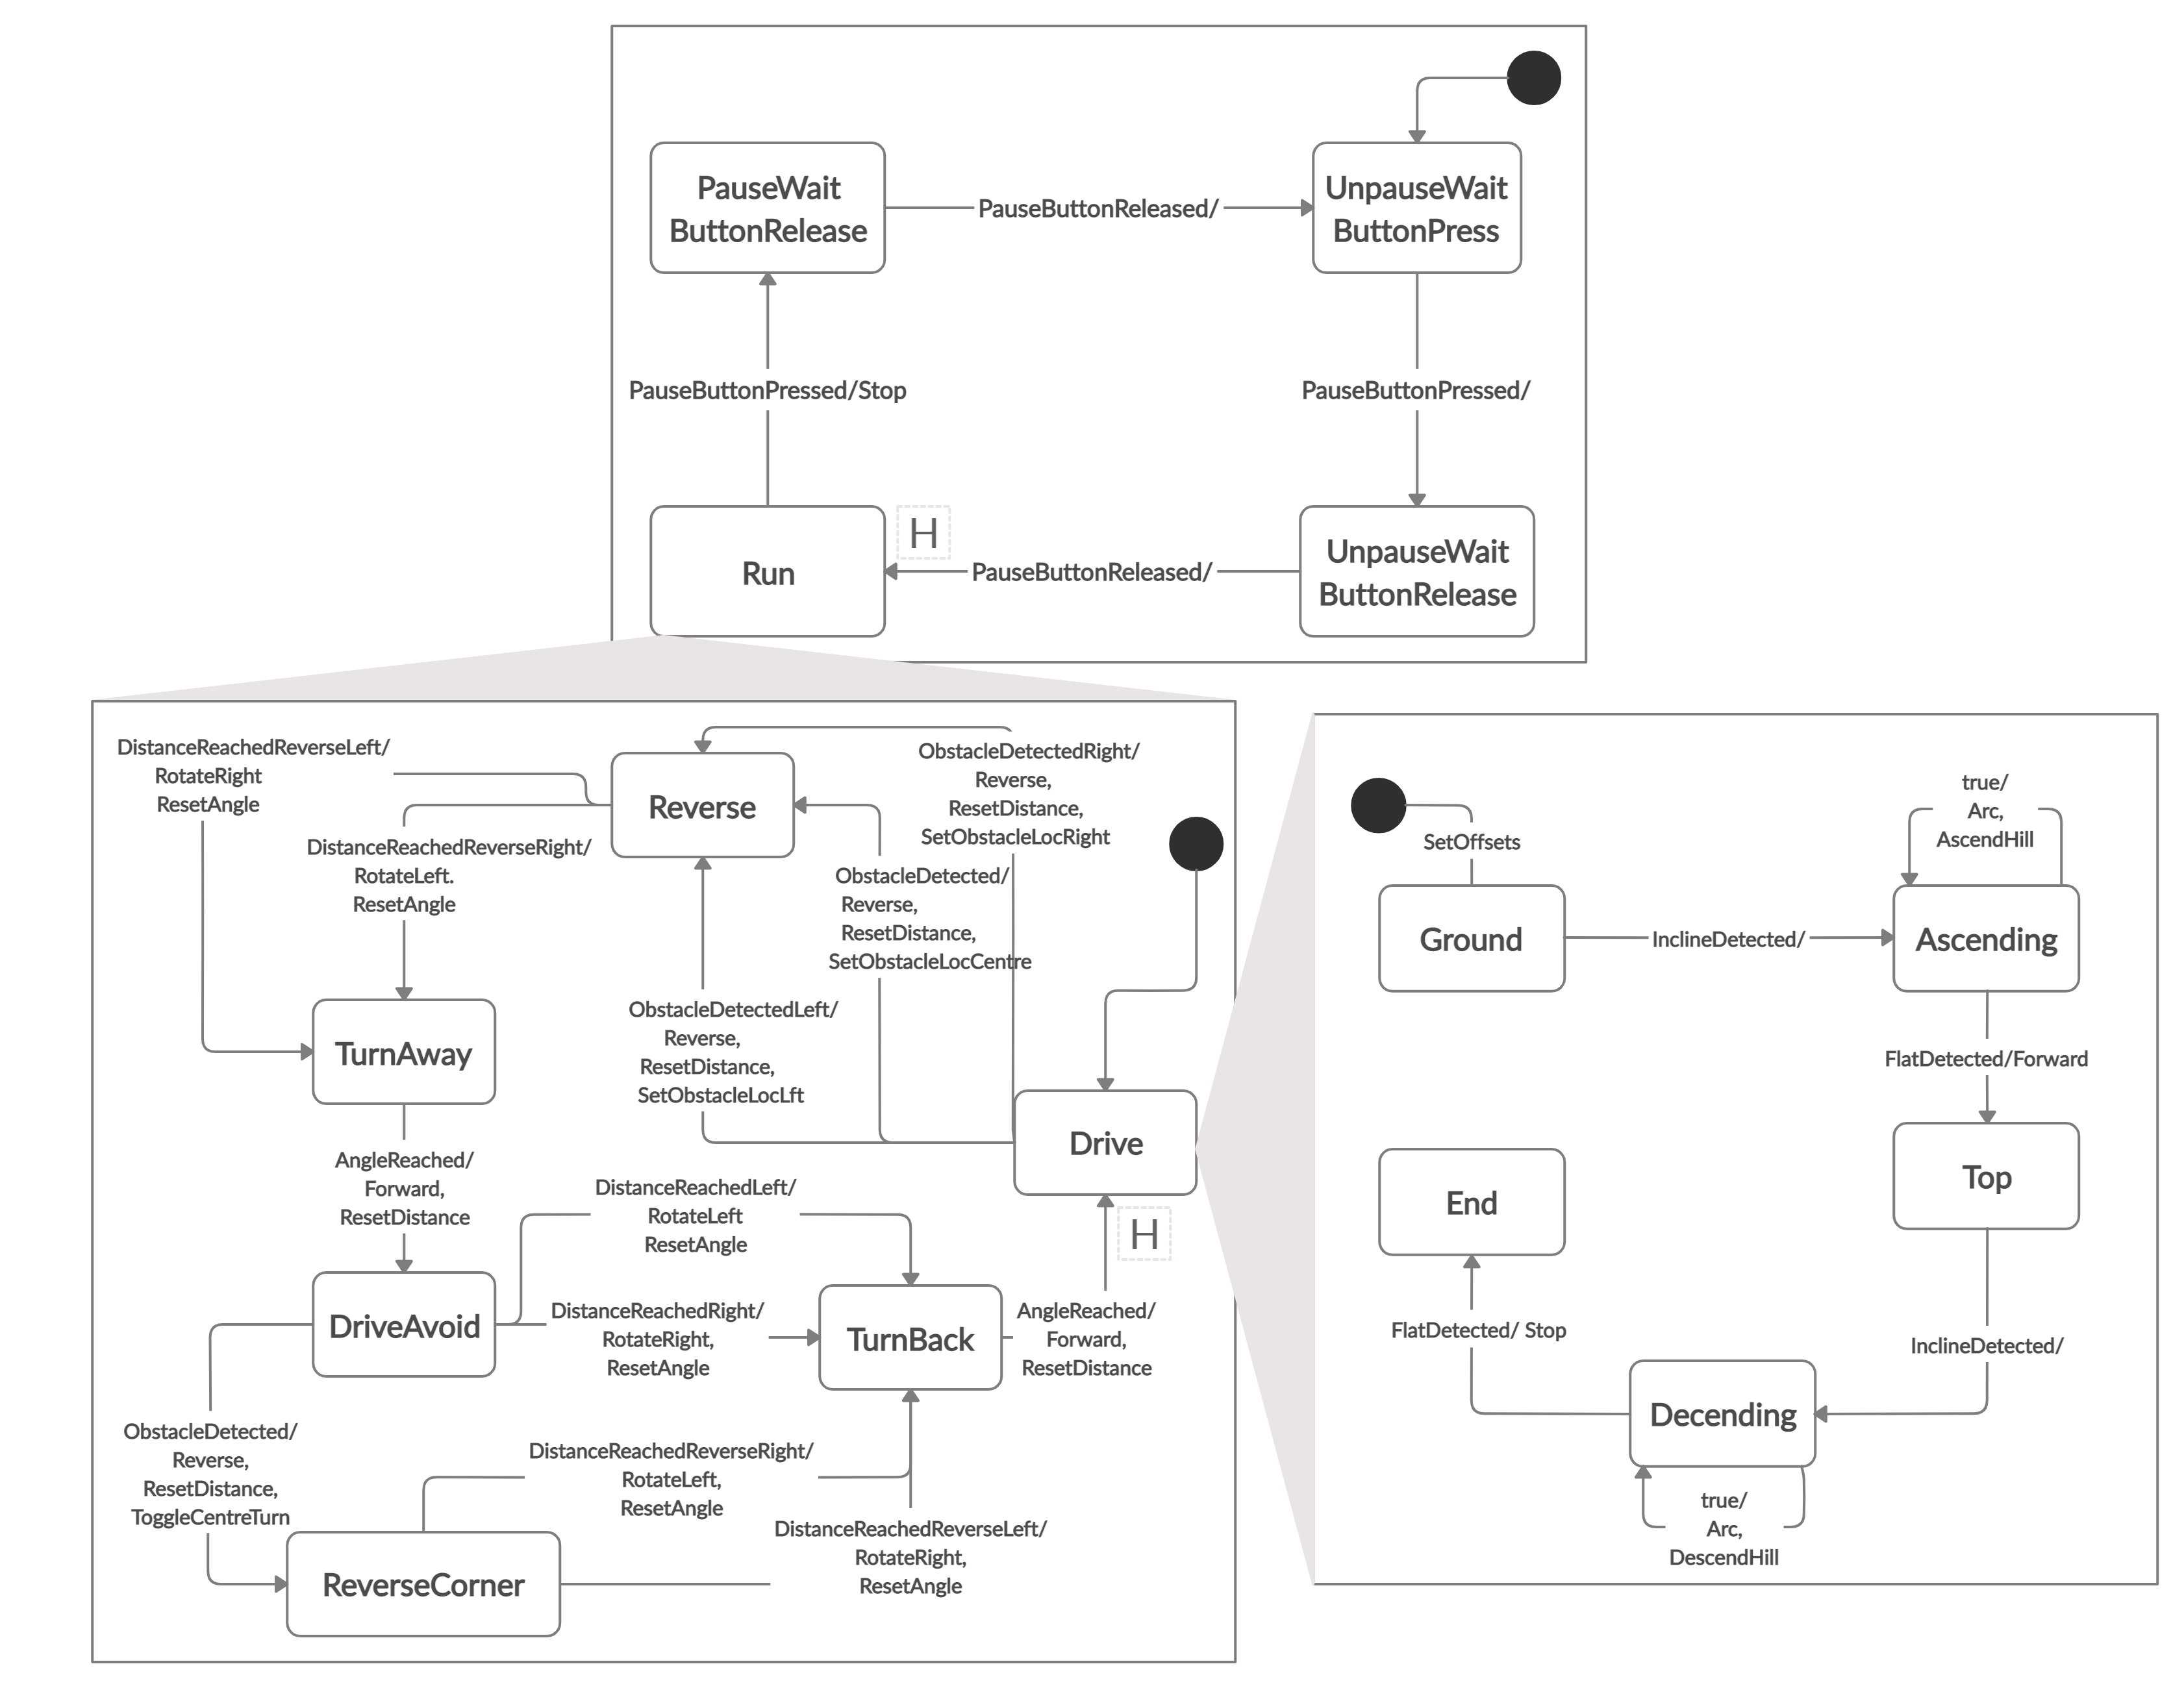
\includegraphics[width=\textwidth]{Finite_State_Machine_v2}
    \caption{Extended State Machine (See Tables \ref{tab:triggers} and \ref{tab:actions} for Trigger and Action definitions)}
    \label{fig:FSM}
\end{figure}

\begin{table}[p]
    \centering
    \begin{tabular}{|c|c|}
        \hline
        Name        & Trigger Definition \\
        \hline\hline
        PauseButtonPressed & \textit{B0} \\
        \hline
        PauseButtonReleased    & $\neg$\textit{B0}  \\
        \hline
        ObstacleDetectedLeft & \textit{cliffLeft} $\lor$ \textit{bumpLeft} $\lor$ \textit{wheelDropLeft}\\
        \hline
        ObstacleDetectedRight & \textit{cliffRight} $\lor$ \textit{bumpRight} $\lor$ \textit{wheelDropRight}\\
        \hline
        ObstacleDetectedCentre & \textit{cliffCentre} $\lor$ \textit{bumpCentre}\\
        \hline
        ObstacleDetected & ObstacleDetectedLeft $\lor$ ObstacleDetectedRight $\lor$ ObstacleDetectedCentre\\
        \hline
        DistanceReached & abs(\textit{netDistance} - \textit{distance}) $\geq$ distanceReachedThreshold\\
        \hline
        DistanceReachedLeft & DistanceReached $\land$ (\textit{obstacleLoc} = LEFT $\lor$ \textit{centreTurn})\\
        \hline
        DistanceReachedRight & DistanceReached $\land$ $\neg$(\textit{obstacleLoc} = LEFT $\lor$ \textit{centreTurn})\\
        \hline
        DistanceReachedReverse & abs(\textit{netDistance} - \textit{distance}) $\geq$ distanceReachedReverseThreshold\\
        \hline
        DistanceReachedReverseLeft & DistanceReachedReverse $\land$ (\textit{obstacleLoc} = LEFT $\lor$ \textit{centreTurn})\\
        \hline
        DistanceReachedReverseRight & DistanceReachedReverse $\land$ $\neg$(\textit{obstacleLoc} = LEFT $\lor$ \textit{centreTurn})\\
        \hline
        AngleReached & abs(\textit{netAngle} - \textit{angle}) $\geq$ 90\\
        \hline
        FlatDetected & abs(\textit{incline)} $<$ flatDetectedThreshold\\
        \hline
        InclineDetected & abs(\textit{incline}) $>$ inclineDetectedThreshold\\
        \hline
    \end{tabular}
    \caption{Trigger Definitions}
    \label{tab:triggers}
\end{table}

\begin{table}[p]
    \centering
    \begin{tabular}{|c|c|}
        \hline
        Name        & Action Definition \\
        \hline\hline
        SetObstacleLocLeft & \textit{obstacleLoc} := LEFT \\
        \hline
        SetObstacleLocRight & \textit{obstacleLoc} := RIGHT \\
        \hline
        SetObstacleLocCentre & \textit{obstacleLoc} := CENTRE \\
        \hline
        ResetDistance & \textit{distance} := \textit{netDistance}\\
        \hline
        ResetAngle & \textit{angle} := \textit{netAngle}\\
        \hline
        Forward & \textit{driveMode} := FORWARD \\
        \hline
        Reverse & \textit{driveMode} := BACKWARD \\
        \hline
        RotateRight & \textit{driveMode} := ROTATE\_RIGHT \\
        \hline
        RotateLeft & \textit{driveMode} := ROTATE\_LEFT \\
        \hline
        Stop & \textit{driveMode} := STOP \\
        \hline
        Arc & \textit{driveMode} := ARC \\
        \hline
        AscendHill & \textit{turnPct} := $-\textit{tiltAngle}/\pi$\\
        \hline
        DescendHill & \textit{turnPct} := $-(\textit{tiltAngle}-\text{sign(\textit{tiltAngle})}\pi)/\pi$\\
        \hline
        ToggleCentreTurn & \textit{centreTurn} := $\neg$ \textit{centreTurn}\\
        \hline
        SetOffsets & \textit{offsets}:= \{\textit{acc.x}, \textit{acc.y}, $1.0-\textit{acc.z}$\}\\
        \hline
    \end{tabular}
    \caption{Action Definitions}
    \label{tab:actions}
\end{table}

\begin{table}[p]
    \centering
    \begin{tabular}{|c|c|c|}
        \hline
        \textit{DriveMode}  & \textit{leftWheelSpeed} & \textit{rightWheelSpeed} \\
        \hline\hline
        FORWARD & SPEED & SPEED \\
        \hline
        BACKWARD & $-$SPEED & $-$SPEED \\
        \hline
        ROTATE\_LEFT & $-$SPEED & SPEED \\
        \hline
        ROTATE\_RIGHT & SPEED & $-$SPEED \\
        \hline
        ARC & $\text{SPEED}(1.0-\textit{turnPct})$ & $\text{SPEED}(1.0+\textit{turnPct})$ \\
        \hline
        STOP & 0 & 0\\
        \hline
    \end{tabular}
    \caption{Output Converter}
    \label{tab:outputs}
\end{table}

%%%% Sims and testing
\newpage
\section{Implementation and Testing}
As alluded to in Section \ref{sec:system}, the simulation environment CyberSim is based on a SolidWorks modelled iRobot instead of the Kobuki. The LabVIEW Robotics Environment Simulator solves ordinary differential equations (ODEs) for the dynamics of the system and renders the outcome into a display dialogue in 3D \cite{labguide}. Our envisioned state machine was built through various iterations through building, simulating, testing on the robot and re-developing.
% potential separate section on simulation/CyberSim? environments .VI etc.

% Simulation results, and how the simulation was shit.
\subsection{LabView vs. C/C++ (Eclipse)}
There were two different ways to implement the state machine on the Kobuki. After implementing parts of the state machine in both LabView and C, it was decided that we would continue using C to implement the state machine. 
%pros and cons of each? in a table?

There are many ways to implement a state machine using C. There was a risk of having unmanageable and unreadable spaghetti code filled with conditional statements. The problem with using a conditional statement approach is that it is difficult to see the difference between states, variables, triggers and actions. An arguably better approach - which we followed - was to define states as structs and triggers/actions as function pointers. This means the main function only needs to look at the current state, check the triggers from the state and if any trigger returns true, perform the actions of that transition. Once the core logic was implemented then adding states was as simple as creating a struct with function pointers to describe transitions. Furthermore, hierarchical state machines were implemented by allowing each state to contain another state. In practice, each refinement was wrapped in a `controller' to handle the variables and behaviour.

\textcolor{blue}{TO DO:\\
- LPF for accelerometer refer to incline plane doc, accuracy of angle calculations etc.\\
- efficiency of code: hierarchical state machines, spaghetti code vs. function pointers\\
- threshold checking for hill climb, simulation vs reality
}

\subsection{Obstacle Avoidance}

\subsection{Hill Climb}
%% harder to test for, accel readings etc. 
% - arc curved movement 
% - kp feedback controller

\section{Validation}
\colorbox{yellow}{Silven}
% some end thing about our performance after it hits challenge requirements
% - final workshop result

\textcolor{blue}{Reasons why it went wrong:\\
- double bumper wasn't tested with the new corner turnaround code\\
- wheeldrop sensors were inactive? may have triggered an incline state\\
- above point explains maybe why ground orientation was lost}

\section{Discussion}
% refer lectures!
% talk about improvements

The low pass filter was not enough to filter out the jumps in the accelerometer values when the Kobuki hits an object and changes speed rapidly. Since the hill climbing algorithm was developed and tested separately, there was not extensive testing of the combined algorithm. In reality and in the simulation, there was a risk of the Kobuki entering the `ascendHill' state after bumping into an object. Figure \ref{fig:debug_incline} demonstrates that even in simulation an incline is detected during a collision - the value $0.68$ is well above the thresholds used and is caused by the large $y$ value of $-0.81$. A low pass filter is able to successfully smooth out the sensor noise, however it is unable to filter out large disturbances to the system. A more sophisticated system is required to ensure the rapid acceleration of the Kobuki does not trigger the hill state transitions.

\begin{figure}[h]
    \centering
    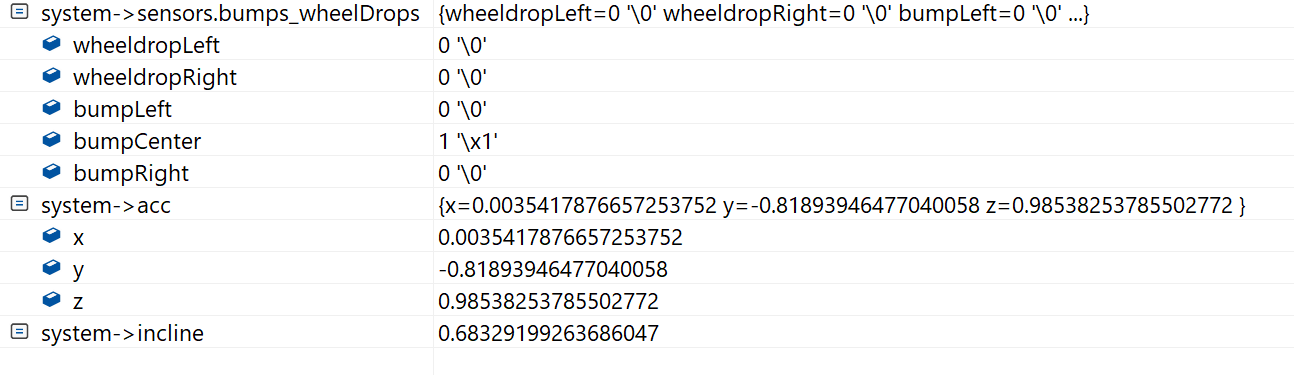
\includegraphics[width=0.8\textwidth]{debug_incline}
    \caption{Debugging Simulation during Collision}
    \label{fig:debug_incline}
\end{figure}

\paragraph{}
Our design fails to describe the behaviour of the system when two events happen in the same update. 

\textcolor{red}{The report must contain (but is not limited to):\\
• a complete FSM diagram (including pause states) of the robot algorithm using the nota- tion covered in the lectures. If you use an Extended state machine, or state refinements, you must show all states, variables and transitions\\
• a basic description of the sensor data available to the myRIO and how it was used in your algorithm\\
• your design procedure (this could include work from earlier workshops)\\
• your testing procedure (this could include simulation data or screenshots)\\
• your validation procedure (this could include reliability or reachability analyses)\\
• the outcome of the run in the final workshop\\
• a discussion section (how you applied knowledge from the lectures, what you would im- prove in the future)
The report is to be no more than 20 pages in length. A marking rubric for the report will be available on LMS.
}

% Appendix
\newpage
\section{Appendix}
\subsection{Source Code}
For all source code and iterations of our Kobuki project code, please refer to our GitHub repository here:\\ \texttt{\url{https://github.com/zeniconcombres/Kobuki}}.\\
The script used to execute the Kobuki state machine can be found here: 
\texttt{\url{https://github.com/zeniconcombres/Kobuki/blob/master/src/C\%20Statechart/KobukiNavigationStateChart.c}}\\
Accompanying the script is the state machine library, which can be found here:
\texttt{\url{https://github.com/zeniconcombres/Kobuki/blob/master/src/C\%20Statechart/KobukiNavigationStateChart.h}}

\medskip

% Bibliography
\bibliographystyle{unsrt}
\bibliography{Bibliography}
% References will occur as they get cited

\end{document}